%%%%%%%%%%%%%%%%%%%%%%%%%%%%%%%%%%%%%%%%%%%%%%%%%%%%%%%%%%%%%%%%%%%%
%% I, the copyright holder of this work, release this work into the
%% public domain. This applies worldwide. In some countries this may
%% not be legally possible; if so: I grant anyone the right to use
%% this work for any purpose, without any conditions, unless such
%% conditions are required by law.
%%%%%%%%%%%%%%%%%%%%%%%%%%%%%%%%%%%%%%%%%%%%%%%%%%%%%%%%%%%%%%%%%%%%

% This theme was based on fibeamer theme 
% If you found any bugs please contact @karlosos
% This repository is hosted on github https://github.com/karlosos/zut-fibeamer/

\documentclass{beamer}
\usetheme[faculty=wi]{fibeamer}
\usepackage[utf8]{inputenc}
\usepackage[
  main=polish,
  polish
]{babel}
\usepackage{hyperref}
\title{Aula 7  - transferindo dados com JSON}
\subtitle{Tópicos especiais em Sistemas}
\author{Prof. Juliana Costa Silva - juliana.silva@up.edu.br}

\usepackage{ragged2e}  % `\justifying` text
\usepackage{booktabs}  % Tables
\usepackage{tabularx}
\usepackage{tikz}      % Diagrams
\usetikzlibrary{calc, shapes, backgrounds}
\usepackage{amsmath, amssymb}
\usepackage{url}       % `\url`s
\usepackage{listings}  % Code listings
\frenchspacing
\begin{document}

%------------------------------------------------------------------------
  \frame[c]{\maketitle}
      \begin{frame}<beamer>
      \frametitle{O que veremos hoje}
      \tableofcontents
    \end{frame}
%------------------------------------------------------------------------
    \section{Revendo...}
    \begin{frame}{Revendo...}{O que já aprendemos?}
      
      \begin{itemize}
            \item Criamos um projeto node;
            \item Configuramos a porta do através do arquivo \textbf{index.js};
            \item Definimos rotas de get da nosso aplicação;
            \item Configuramos nodemon no ambiente dev;
       \end{itemize}
     \end{frame}
%------------------------------------------------------------------------
\section{Introdução}
    \begin{frame}[label=lists]{Post}
    \begin{exampleblock}{Qual a função do POST}
        	\begin{itemize}
	\item Enviar dados ao servidor;
	\item Receber dados do usuário;
        	\end{itemize}
      \end{exampleblock}
    \end{frame}
%------------------------------------------------------------------------
\section{POST}
    \begin{frame}[label=lists]{Requisição}

% \begin{columns}[onlytextwidth]
%        \column{.5\textwidth}
         Vamos ler as informações enviadas através do POST.
         \begin{itemize}
         \item No arquivo \textbf{movimento.js};
         \item Vamos acrescentar \alert{console.log(req.body)}, o body relativo ao corpo do site, e header seria o cabeçalho.
         \end{itemize}
          \vspace{0.5cm}
          No arquivo \textbf{movimento.js} acrescente o código entre as linhas 6 e 7 no início do post
%
%        \column{.5\textwidth}
	            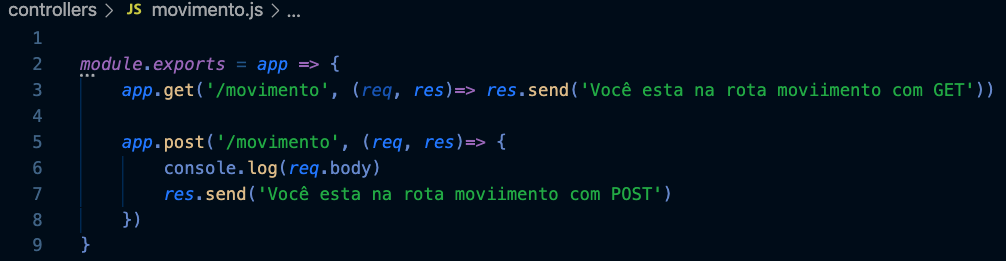
\includegraphics[width=110mm]{resources/aula5_1.png}\\
            \tiny{\textbf{Fonte:} O autor}
%      \end{columns}
    \end{frame}

 %------------------------------------------------------------------------
    \begin{frame}[label=lists]{Postman}
   No área de trabalho do Postman faremos configurações da requisição: 
   \begin{itemize}
       \item Tipo de conteúdo;
       \item Tamanho da requisição;
       \item Qual user, etc.
       \end{itemize}
       Neste momento trabalharemos apenas com "content-type",  tipo do conteúdo.
	\begin{alertblock}{contet-type}
		O contet-type padrão é o "urlencoded", que está relacionado aos formulários produzidos em HTML. \\
	Na aba "body" na área de trabalho do Postman enviaremos essa requisição com o nome "Juliana".
	\end{alertblock}
    \end{frame}
     %------------------------------------------------------------------------
    \begin{frame}[label=lists]{Funciona?}
	\begin{exampleblock}{Conversando com a requisição}
	\begin{itemize}
	\item Ao observarmos nosso console, receberemos \alert{undefined};
	\item Isso ocorre porque nossa requisição não sabe ler nosso body;
	\item Para que a aplicação conseguia entender a requisição, instalaremos uma biblioteca chamada \textbf{body-parser}, 
	\item Esta biblioteca tem a função converter as requisições para algo que seja legível no JavaScript.
	\end{itemize}
	\end{exampleblock}
    \end{frame}
   
 %------------------------------------------------------------------------
 \section{Instalando o Body-Parser}
    \begin{frame}[label=lists]{npm-install}
    Na linha de comando escreveremos \alert{npm install body-parser}.\\
	\begin{exampleblock}{Editando CustomExpress.js}
		\begin{itemize}
			\item Dentro de customExpress.js, vamos alterar como nosso servidor opera;
			\item As traduções não serão apenas para essa requisição específica, mas um modo de operação geral;
			\item Importaremos a biblioteca bodyParser;
			\item Então pediremos para que app utilize (use()) essa biblioteca específica.;
			\item Existem muitas maneiras de realizar essa tradução de requisição, e neste caso utilizaremos o urlenconded com a opção extended: true para que tudo opere normalmente;
		\end{itemize}
	\end{exampleblock}
	     \end{frame}
    %------------------------------------------------------------------------
    \begin{frame}[label=lists]{Enviando dados POSTMAN}
		\begin{itemize}
			\item Escolha a opção POST no POSTMAN;
			\item Selecione "body" na sub-guia e urlenconded;
			\item Como na imagem abaixo preencha algum dado, com \textbf{chave} e \textbf{valor}.
		\end{itemize}
		\begin{center}
    		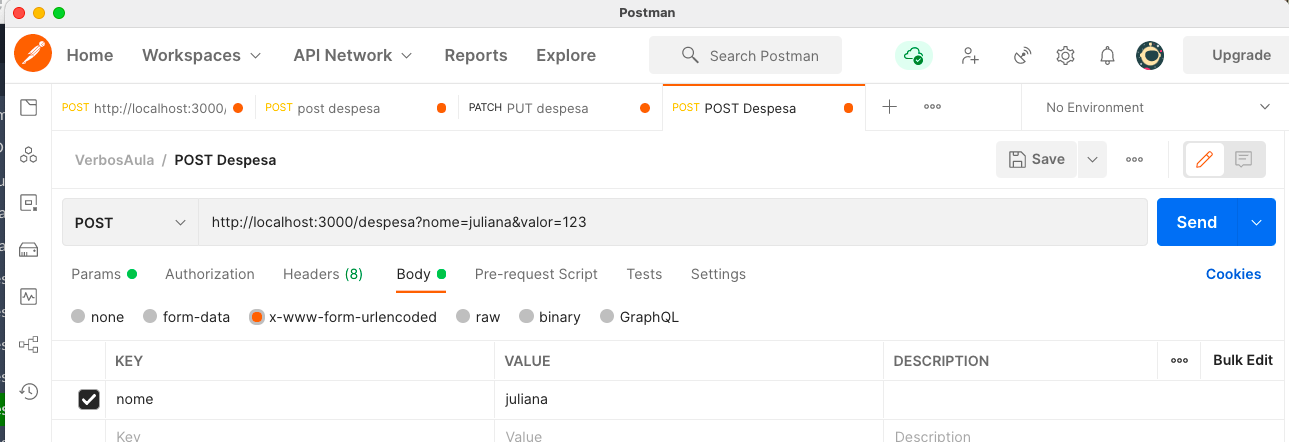
\includegraphics[width=100mm]{resources/aula5_4.png}\\
	        \tiny{ Código no postman \textbf{Visualização postman}. \textbf{Fonte:} O autor}
	 \end{center}
	     \end{frame}
    %------------------------------------------------------------------------
    \begin{frame}[label=lists]{CustomExpress.js}
	\begin{center}
    		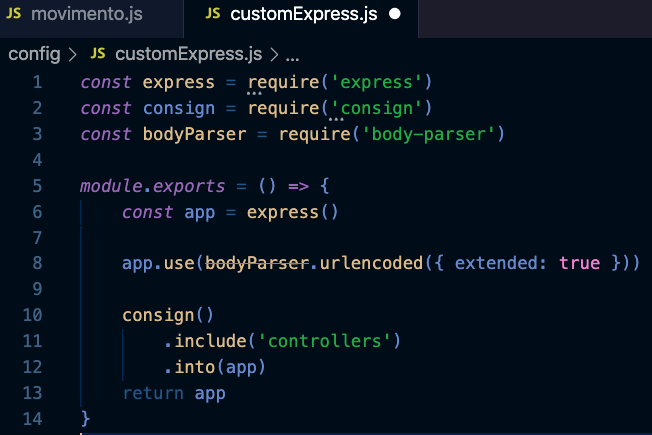
\includegraphics[width=100mm]{resources/aula5_2.png}\\
	        \tiny{ Código no arquivo \textbf{customExpress.js}. \textbf{Fonte:} O autor}
	 \end{center}
    \end{frame}
 %------------------------------------------------------------------------
    \begin{frame}[label=proof]{Repensando...}
    \begin{alertblock}{Só para browser?}
	\begin{itemize}
	\item Ao enviarmos a requisição veremos em nosso console o nome "juliana", o que significa que a tradução foi realizada \cite{nodejs2022api}. 
	\item Contudo, a API nem sempre é feita só para browser, então não vamos enviar conteúdos apenas por um formulário.
	\item Algo muito como de se realizar no frond-end é coletar os dados de um formulário, manipular-los de alguma maneira, transformá-los em objeto json e então realizar o envio para o back-end.
	\item Portanto para que a nossa API possa ser consumida por outros serviços, adicionaremos essa especificidade do json \cite{postman2022}.
	\end{itemize}
	\end{alertblock}
    \end{frame}
 %------------------------------------------------------------------------
    \begin{frame}{CustomExpress.js}
         \begin{center}
    	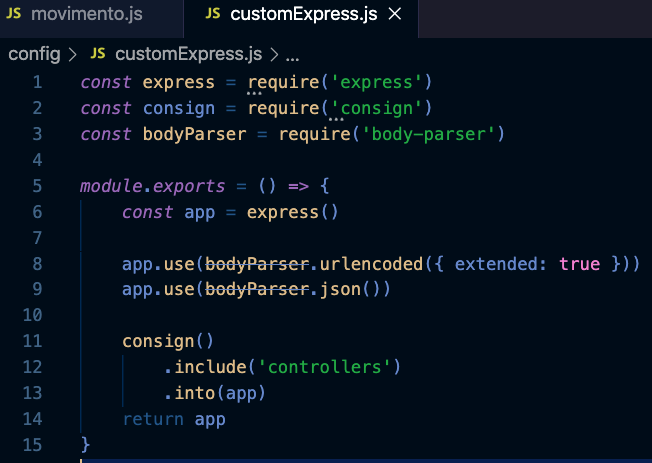
\includegraphics[width=100mm]{resources/aula5_3.png}\\
        \tiny{ Código no arquivo \textbf{customExpress.js}. \textbf{Fonte:} O autor}
     \end{center}   
    \end{frame}
  %-----------------------------------------------------------------------------
  \section{Atividade}
  \begin{frame}{Atividade de aula}
   \begin{enumerate}
     \item Desenvolva a rota \textbf{carteiras};
     \item Essa rota cuidará do cadastro de diferentes carteiras no orçamento pessoal;
     \item Desenvolva o GET  e POST dessa rota, e identifique os dados em formato JSON para cadastrar uma carteira; 
     \item Envie como respostas o código de carteira.js e o JSON enviado via Postman nos testes (impresso no console).
   \end{enumerate}
  \end{frame}
%------------------------------------------------------------

%------------------------------------------------------------------------
\section{Referências}
\begin{frame}{Referências}%[allowframebreaks]
\small
\begin{center}
\tiny
\bibliographystyle{apalike}
\bibliography{ref_aula}
\end{center}
\end{frame}
  
\end{document}